\subsection{Mechanical Interaction}
The mechanical design has three parts:
\begin{enumerate}
    \item a \textbf{custom grip} that replaces the factory AR-15 grip and
    houses the electronics, battery, and RFID antenna
    \item an \textbf{actuator mount} that locates the micro stepper in the fire
    control pocket of the lower receiver
    \item a \textbf{blocking member} driven by the motor that physically
    prevents the fire control group from releasing the hammer
\end{enumerate}

To understand the innovation behind the blocking member takes some understanding of the original function of the 
    AR-15 fire control group(trigger, hammer, sear, and safety). To fire a round the trigger must be pulled, the angle the 
    trigger is brought to in its movement releases the hold it had on the spring loaded hammer. The freed hammer slams against
    onto a hook called the disconnector which holds the hammer until the trigger is back to its ready position it was in before 
    firing the last round. The safety on the AR-15 is a physical barrier to the trigger. When is the safe position the trigger
    is physically blocked from movement thus preventing the hammer from moving and the overall firing of the gun. The design 
    of our safety takes advantage of the mechanical blocker of the AR-15's native safety selector. To create the most widely 
    applicable design we focused on locking the native safety in place until an authorized user is recognized.

\subsection{Component Selection}

\begin{table}[H]
\centering
\caption{Components in the Smart Trigger system}
\label{tab:Bill_of_Materials}
\scriptsize
\setlength{\tabcolsep}{3pt}
\begin{tabularx}{\columnwidth}{|l|l|>{\raggedright\arraybackslash}X|}
\hline
\textbf{Part Number} & \textbf{Short Name} & \textbf{Short Description} \\ \hline
Pi Pico W & Pico         & Microcontroller and central brain \\
SAA1042   & Motor Driver & Stepper motor driver \\
RDM6300   & RFID Reader  & RFID reader and translator \\
ANT1      & Antenna      & Custom wound antenna tuned to 125\,kHz \\
M1        & Motor        & Stepper motor to rotate shaft \\
R1        & R            & 47\,k$\Omega$ resistor \\
C1        & C            & 100\,nF capacitor \\ \hline
\end{tabularx}
\end{table}



\subsection{Main Board (PCB)}

\subsubsection{Rationale for a Custom PCB}

The project imposed a strict size constraint on the electronics enclosure: the usable inner cavity of the pistol grip measures 88.8\,mm from top to bottom, 21.9\,mm wide, and 45.0\,mm across.
A custom printed circuit board (PCB) would integrate all components listed in Table \ref{tab:Bill_of_Materials} into a compact form. 
A custom design also offered greater control over the system, since unnecessary components could be removed and only the required circuitry 
selected from each of the commercial development boards. 
Finally, a single integrated board would simplify installation for the end user compared with a multi-board assembly.

\subsubsection{Design Process and Change in Approach}

With these constraints in mind, we began by reverse engineering the RDM6300 RFID module, which serves as the interface between the Raspberry Pi Pico microcontroller and the RFID tag. 
We recreated the circuit in KiCad, a PCB design tool, and started to validate it through simulation in LTSpice. 
The resulting design is shown in Figure \ref{fig:PCB_Design_1}. 

\begin{figure} [h]
    \centering
    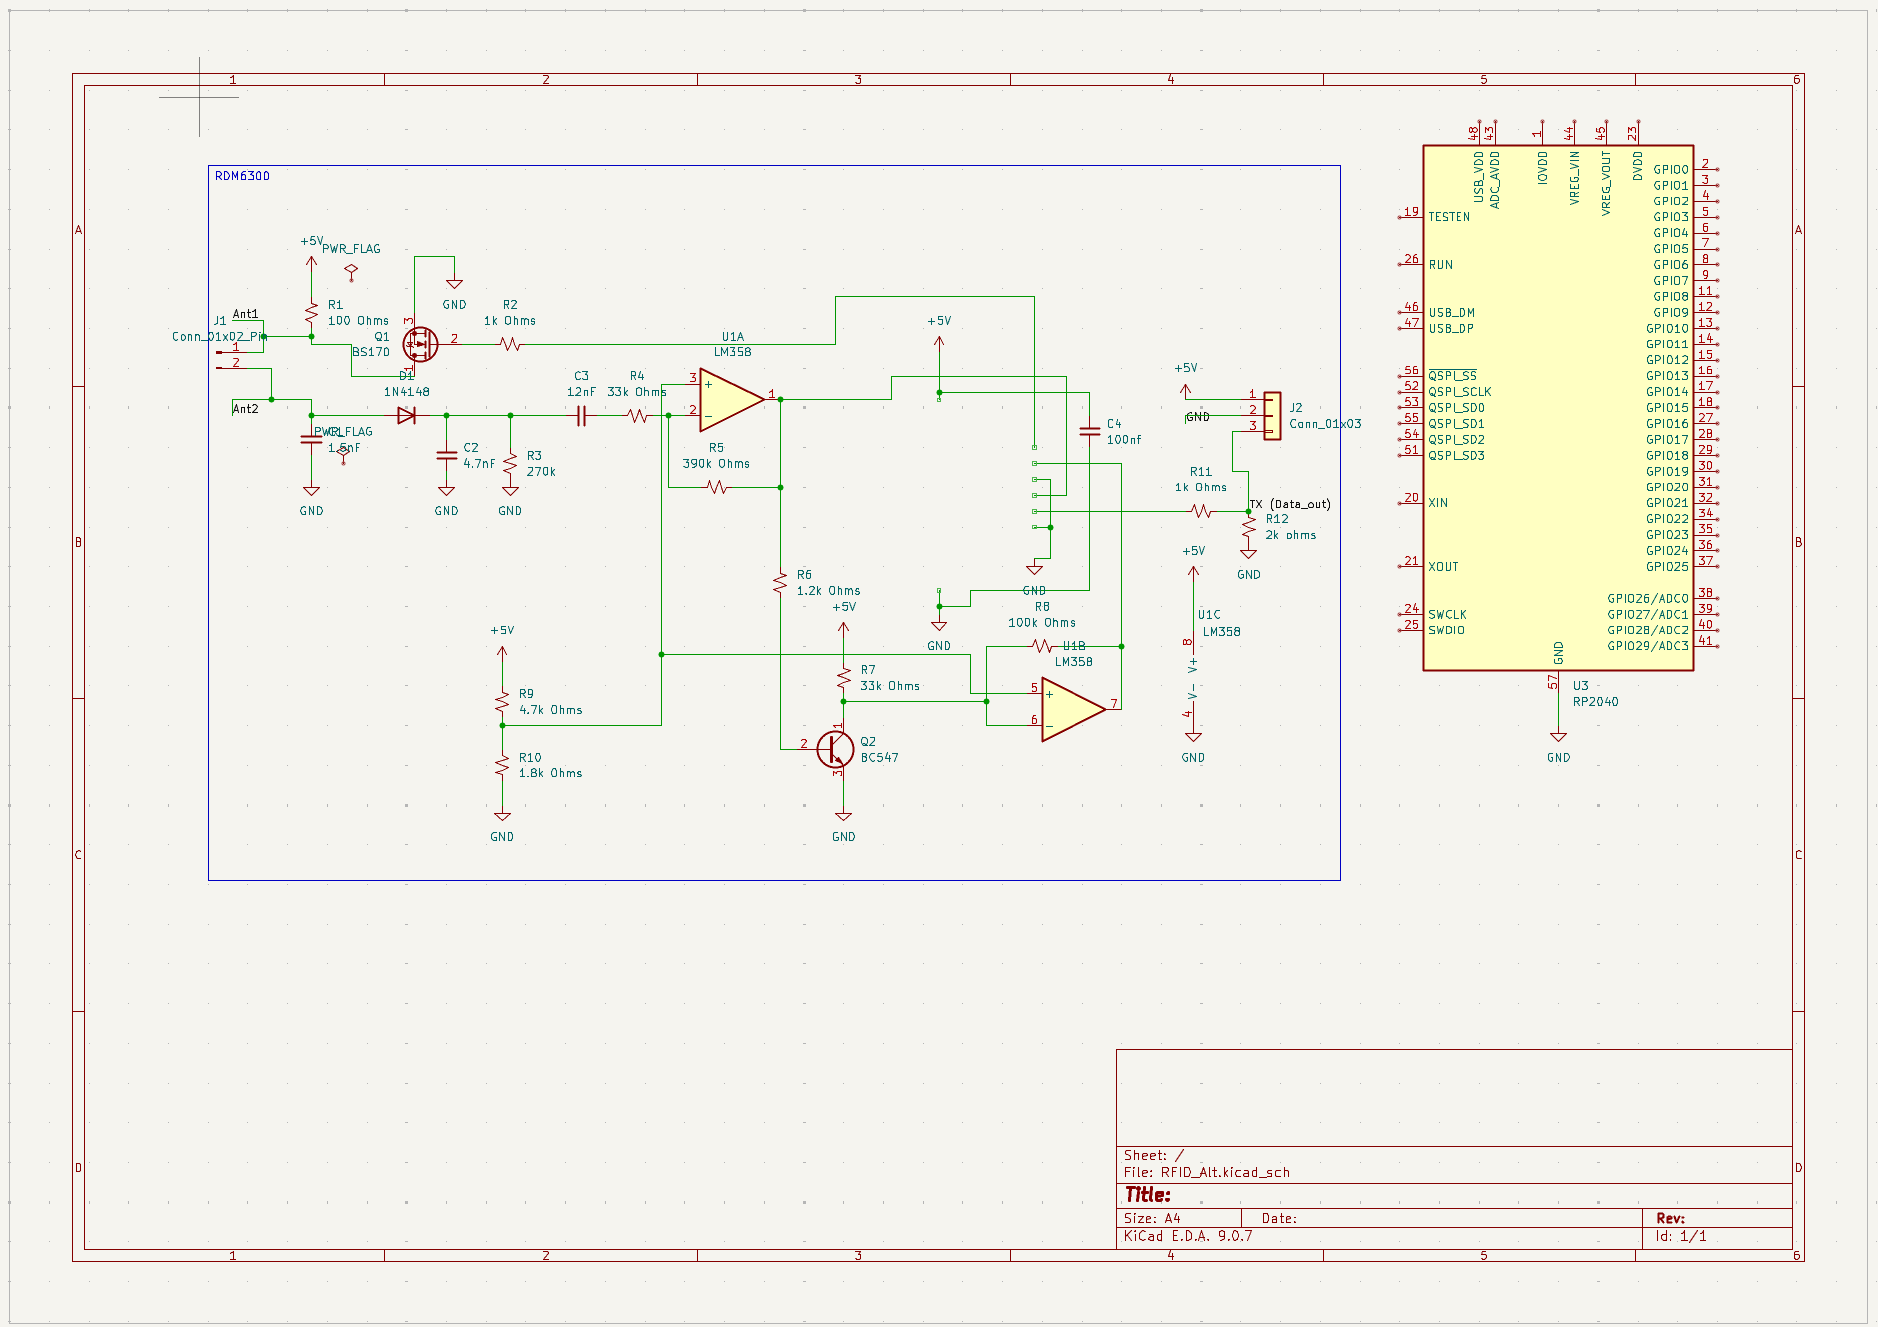
\includegraphics[width=0.4\textwidth]{Images/PCB_Design_1.png}
    \caption{First Iteration of the Custom PCB Design. The design integrates the RDM6300 RFID module, 
    the SAA1042 stepper motor driver, and the Raspberry Pi Pico microcontroller into a single board.}
    \label{fig:PCB_Design_1}
\end{figure}

This design would have allowed us to remove the RP2040 from its development board and mount it directly on the custom PCB, 
eliminating the many GPIO pins we did not intend to use.

Before fabricating and testing the board, however, the team questioned whether the fine-pitch leads of the RP2040 could be reliably hand soldered. 
Commercial manufacturers typically place such components using processes such as stencil-based solder paste application with reflow, or 
thermocompression bonding, neither of which was available to us. Given the project schedule and the risk of failing to mount the chip, we elected 
to pursue a simpler design.

\subsubsection{Tradeoffs of the Revised Design}

Although each of the existing boards fit within the grip, they would not be held securely in place. We therefore changed the role of the PCB to that of a 
perfboard-style central hub that interconnects the individual boards. This decision involved several tradeoffs. The perfboard approach 
retains unused features, including GPIO pins, clock circuitry, and UART pins. The boards must also be arranged to fit within the grip, 
making the assembly less compact than a custom PCB that integrates their functions. However, this approach required no additional parts, 
since all components were already in hand, and its lower complexity improved the likelihood of delivering a working product by the deadline.

The current design is shown in Figure \iffalse \ref{fig:PCB_Design_2}\fi. The board is configured to sandwich the Raspberry Pi Pico microcontroller on one 
side with the motor driver on the opposite side. The RDM6300 sits directly below the motor driver and is mounted through solder points that 
accept the short portion of its header pins, forming a compact stack of boards.

\subsection{RFID Board (RDM6300)}

\subsubsection{How RFID Technology Works}

 RFID (Radio Frequency Identification) requires two components to communicate: a reader and a tag. 
 The reader consists of an antenna and a transceiver, while the tag consists of an antenna and a 
 transponder \cite{kaur2011rfid}. Tags are classified as either active or passive. An active tag 
 contains a battery and can transmit its signal over long distances, whereas a passive tag has no 
 battery and can transmit only when it is within range of a reader. The reader's antenna emits a 
 radio frequency signal that powers the passive tag, and the strength of this signal depends on the 
 number of coil turns in the antenna. Once powered, the tag transmits its unique ID back to the reader. 
 The reader then decodes this signal and forwards it to a microcontroller for processing.

\subsubsection{How we implemented RFID in our system}

 \begin{figure} [h]
    \centering
    % trim crops the PDF's white margins so the diagram can be 25% larger and still fit the column
    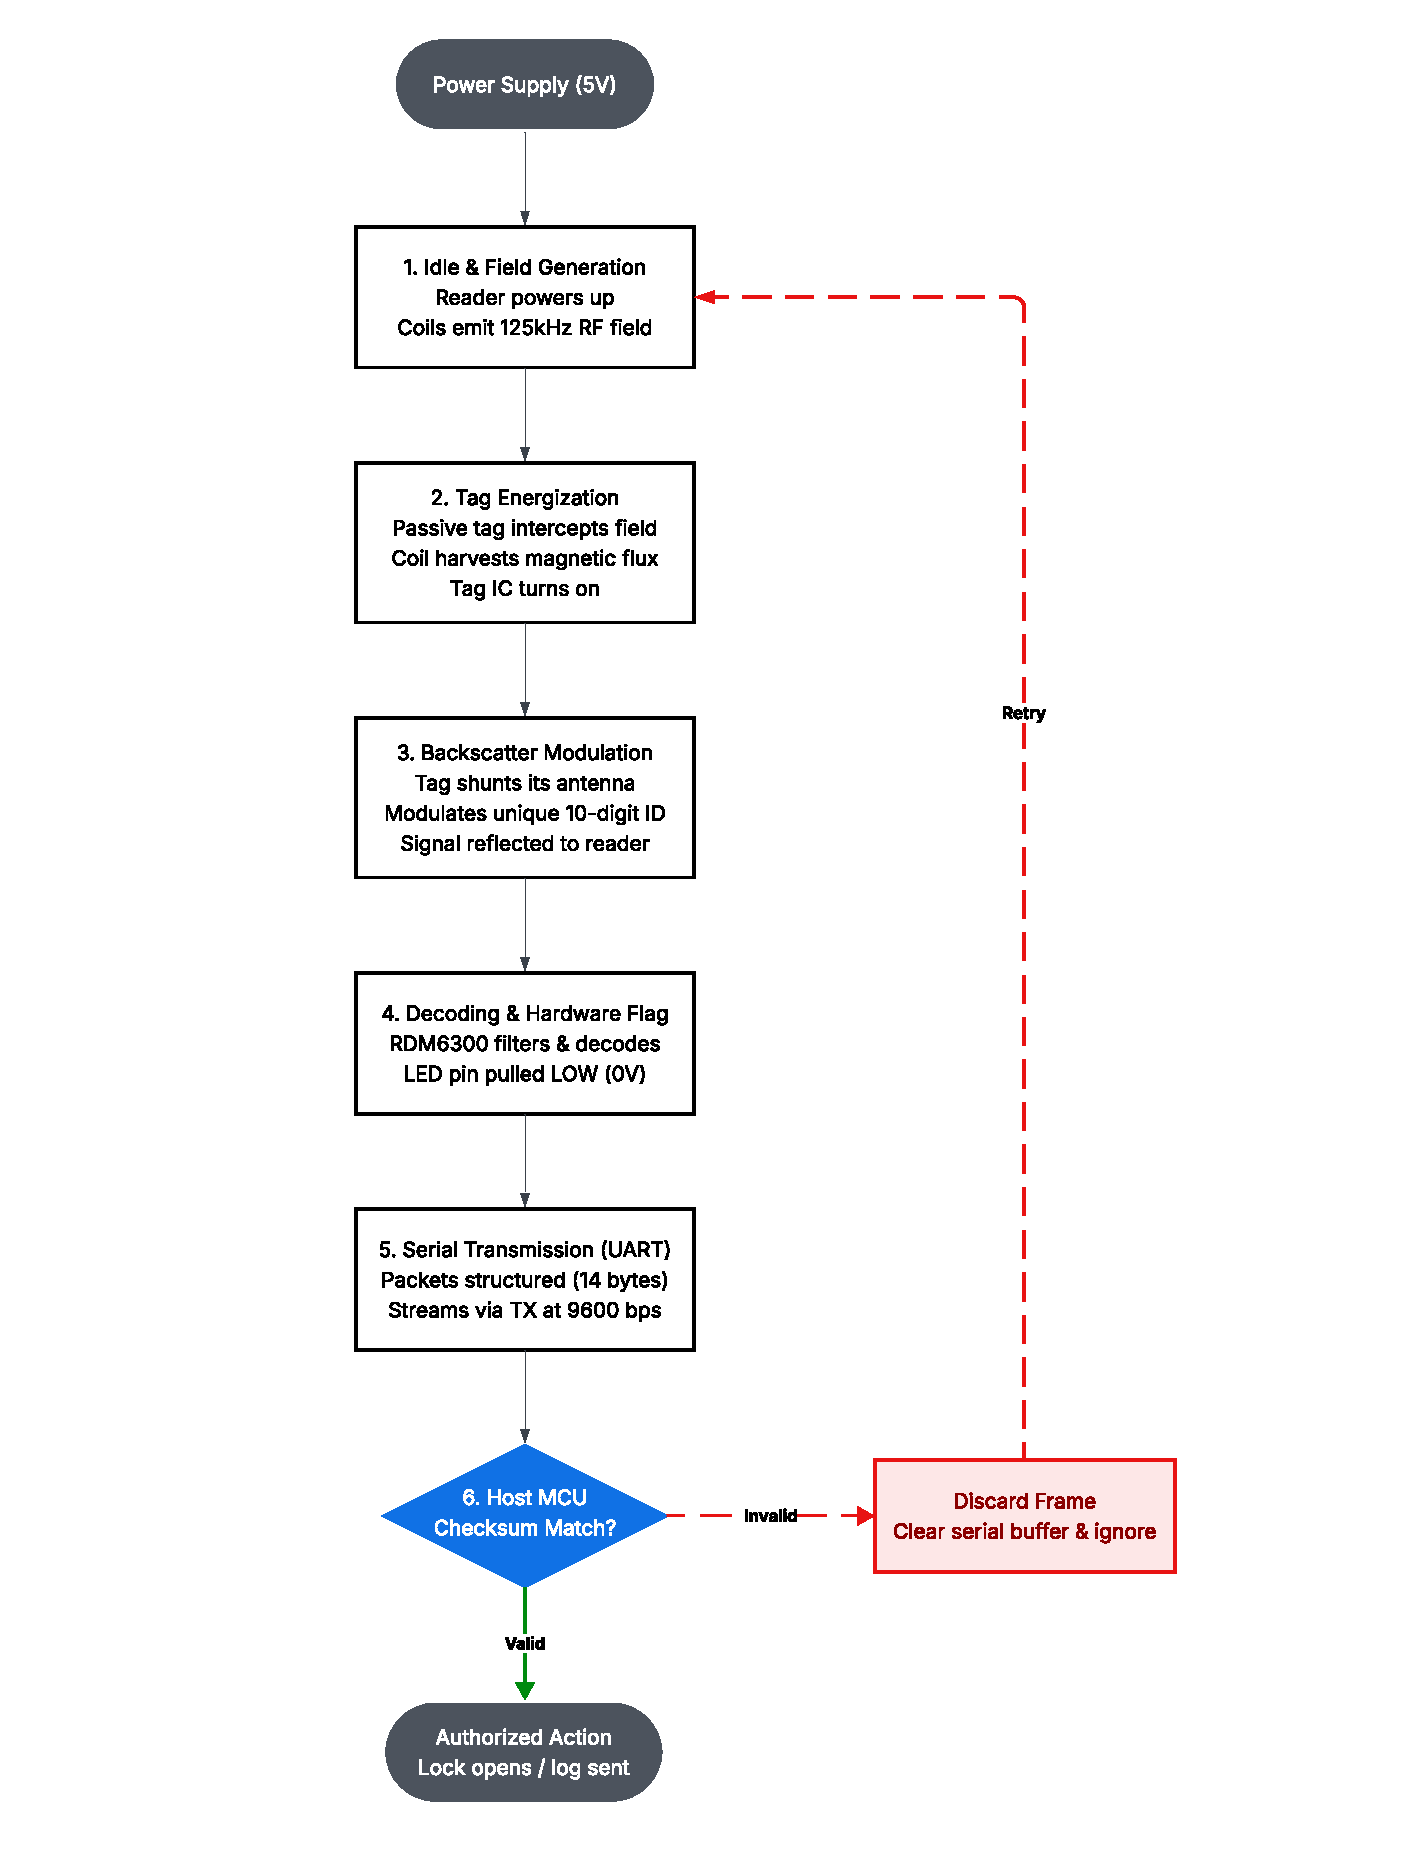
\includegraphics[trim=162 27 102 10, clip, width=0.76\columnwidth]{Images/RDM6300_V.pdf}
    \caption{A flow diagram of the RDM6300 RFID module. The module reads the RFID tag and translates its signal into a UART serial output for the Raspberry Pi Pico.}
    \label{fig:RDM6300_Flowchart}
\end{figure}

 This project uses a passive tag because the system does not require long-range communication, and passive tags are lower in cost 
 and power consumption. The reader antenna is custom wound and tuned to 125 kHz. The accepted tag IDs are currently hardcoded in the 
 firmware. When a tag enters the reader's range, the RDM6300 module reads the tag and converts its signal into a UART serial output, 
 which is sent to the Raspberry Pi Pico. The Pico compares the received tag ID against the list of accepted IDs. If the ID matches, 
 the Pico signals the motor driver to unlock the safety. If the ID is not accepted, no action is taken and the safety remains locked. 
 This process is illustrated in Figure \ref{fig:RDM6300_Flowchart}.


\subsection{Micro Stepper Motor \& Driver Board (SAA1042)}

Stepper motors are a type of brushless DC motor that rotate when current is driven through their windings. 
Unlike a standard DC motor, which rotates continuously when a current is applied, a stepper motor rotates 
in discrete angular increments, or steps. Stepper motors are generally divided into two types. Permanent magnet 
stepper motors produce rotation through the interaction between a permanent magnet and energized electromagnets. 
Variable-reluctance stepper motors, in contrast, contain no permanent magnet and rely solely on electromagnetic forces to produce rotation.

\begin{figure} [h]
    \centering
    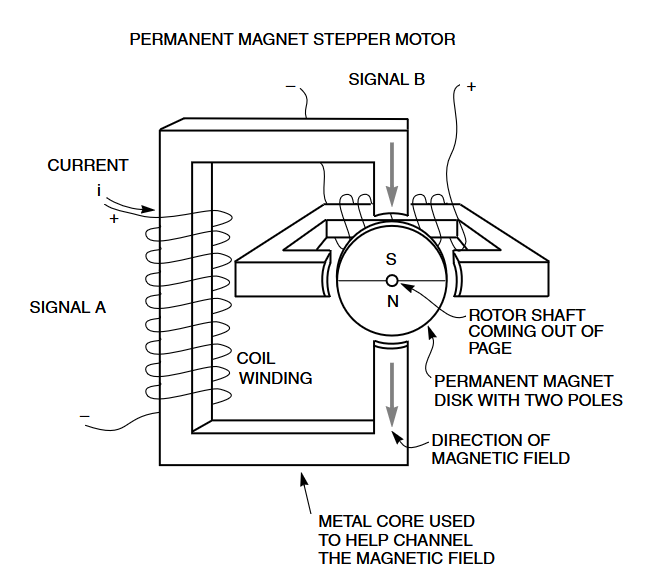
\includegraphics[width=\columnwidth]{Images/Stepper_Motor_Diagram.png}
    \caption{A flow diagram of the stepper motor and driver board. Taken from \cite{grant2005quick}}
    \label{fig:Stepper_Motor_Flowchart}
\end{figure}

Each motor consists of a stator, a rotor with a shaft, and coil windings, as shown in Figure \ref{fig:Stepper_Motor_Flowchart}. 
When current is passed through the coil windings, it generates a magnetic field that interacts with the rotor and 
causes it to rotate. The direction of rotation is determined by the direction of the current through the windings. 
The motor used in this design is a permanent magnet stepper motor.


